%% ----------------------------------------------------------------
%% Report.tex
%% ---------------------------------------------------------------- 
\documentclass{ecsreport}      % Use the Report Style
\graphicspath{{../Figures/}}   % Location of your graphics files
\usepackage{natbib}            % Use Natbib style for the refs.
\hypersetup{colorlinks=true}   % Set to false for black/white printing
\input{Definitions}            % Include your abbreviations
%% ----------------------------------------------------------------
\begin{document}
\frontmatter
\title      {An Investigation into \dots}
\authors    {\texorpdfstring
             {\href{mailto:hl13g10@ecs.soton.ac.uk}{Henry S. Lovett}}
             {Henry S. Lovett}
            }
\addresses  {\groupname\\\deptname\\\univname}
\date       {\today}
\subject    {}
\keywords   {}
\maketitle
\begin{abstract}
This work is all about \dots
\end{abstract}
\tableofcontents
\listoffigures
\listoftables
\lstlistoflistings
\listofsymbols{ll}{$w$ & The weight vector}
\acknowledgements{Thanks to no one.}
\dedicatory{To \dots}
\mainmatter
%% ----------------------------------------------------------------
%% ----------------------------------------------------------------
%% Introduction.tex
%% ---------------------------------------------------------------- 
\chapter{Introduction} \label{Chapter:Introduction}
%The Introduction to my Report \dots

%The initial idea of the project was taken from Pirobot(\cite{Pirobot}).
%
%\inote{what it will do. Define everything. Use. Very general}
%General - mapping robots. 
%
%stereovision - uses etc.
%
%other similar projects
%
%why mine is important 


This report documents the design, testing and building of a stereoscopic mapping robot. The end product will be a small, two wheeled robot with a roller ball, that will autonomously search and map an unknown area and produce an occupancy map of the searched area. 

An occupancy map is a representation of an area where a location is given a value of either \textit{free, occupied} or \textit{unkown} (\cite{thrun2003learning}).  Three dimensional occupancy maps can also be generated, such as the OctoMap (\cite{octomap}). Objects can also be tracked using an occupancy map and statistics (\cite{Fleuret:OccupancyMap}). 

The purpose of a mapping robot is to build a representation of the area around it. This then facilitates the use of any application that requires prior knowledge of the area. One algorithm that is used to build up an occupancy map is the S.L.A.M. algorithm (\cite{Thrun:SLAM}) and is used in other mapping robots(\cite{Se:MappingRobot}). Accurate mapping robots tend to use laser range finders (\cite{Ruhnke:LaserMapping}).

Stereoscopy in computer vision is the ability to calculate the locations and depths using images from two or more cameras, which are used to triangulate and estimate distances (\cite{Saxena:DepthEstimation}). By using two cameras on the same plane, separated by a set horizontal distance, the depth of the observed scene can be perceived by the system.

Stereovision is a small section of computer vision which is widely used in many applications, including Microsoft's Xbox Kinect (\cite{Microsoft:Kinect}), where stereo vision is used to locate a game player in order to use their movements to control the game. \cite{Mrovlje:Distance_Stereoscopic} uses stereovision to be able to locate the distance to a marker.

The stereovision mapping robot discussed in this report is a low cost alternative to other robots which use laser range finders or high quality cameras (\cite{Se:MappingRobot}). The robot will use the base seen in figure \ref{fig:RobotBase} and use two OmniVision OV7670 cameras delivering QVGA format images.

\begin{figure}
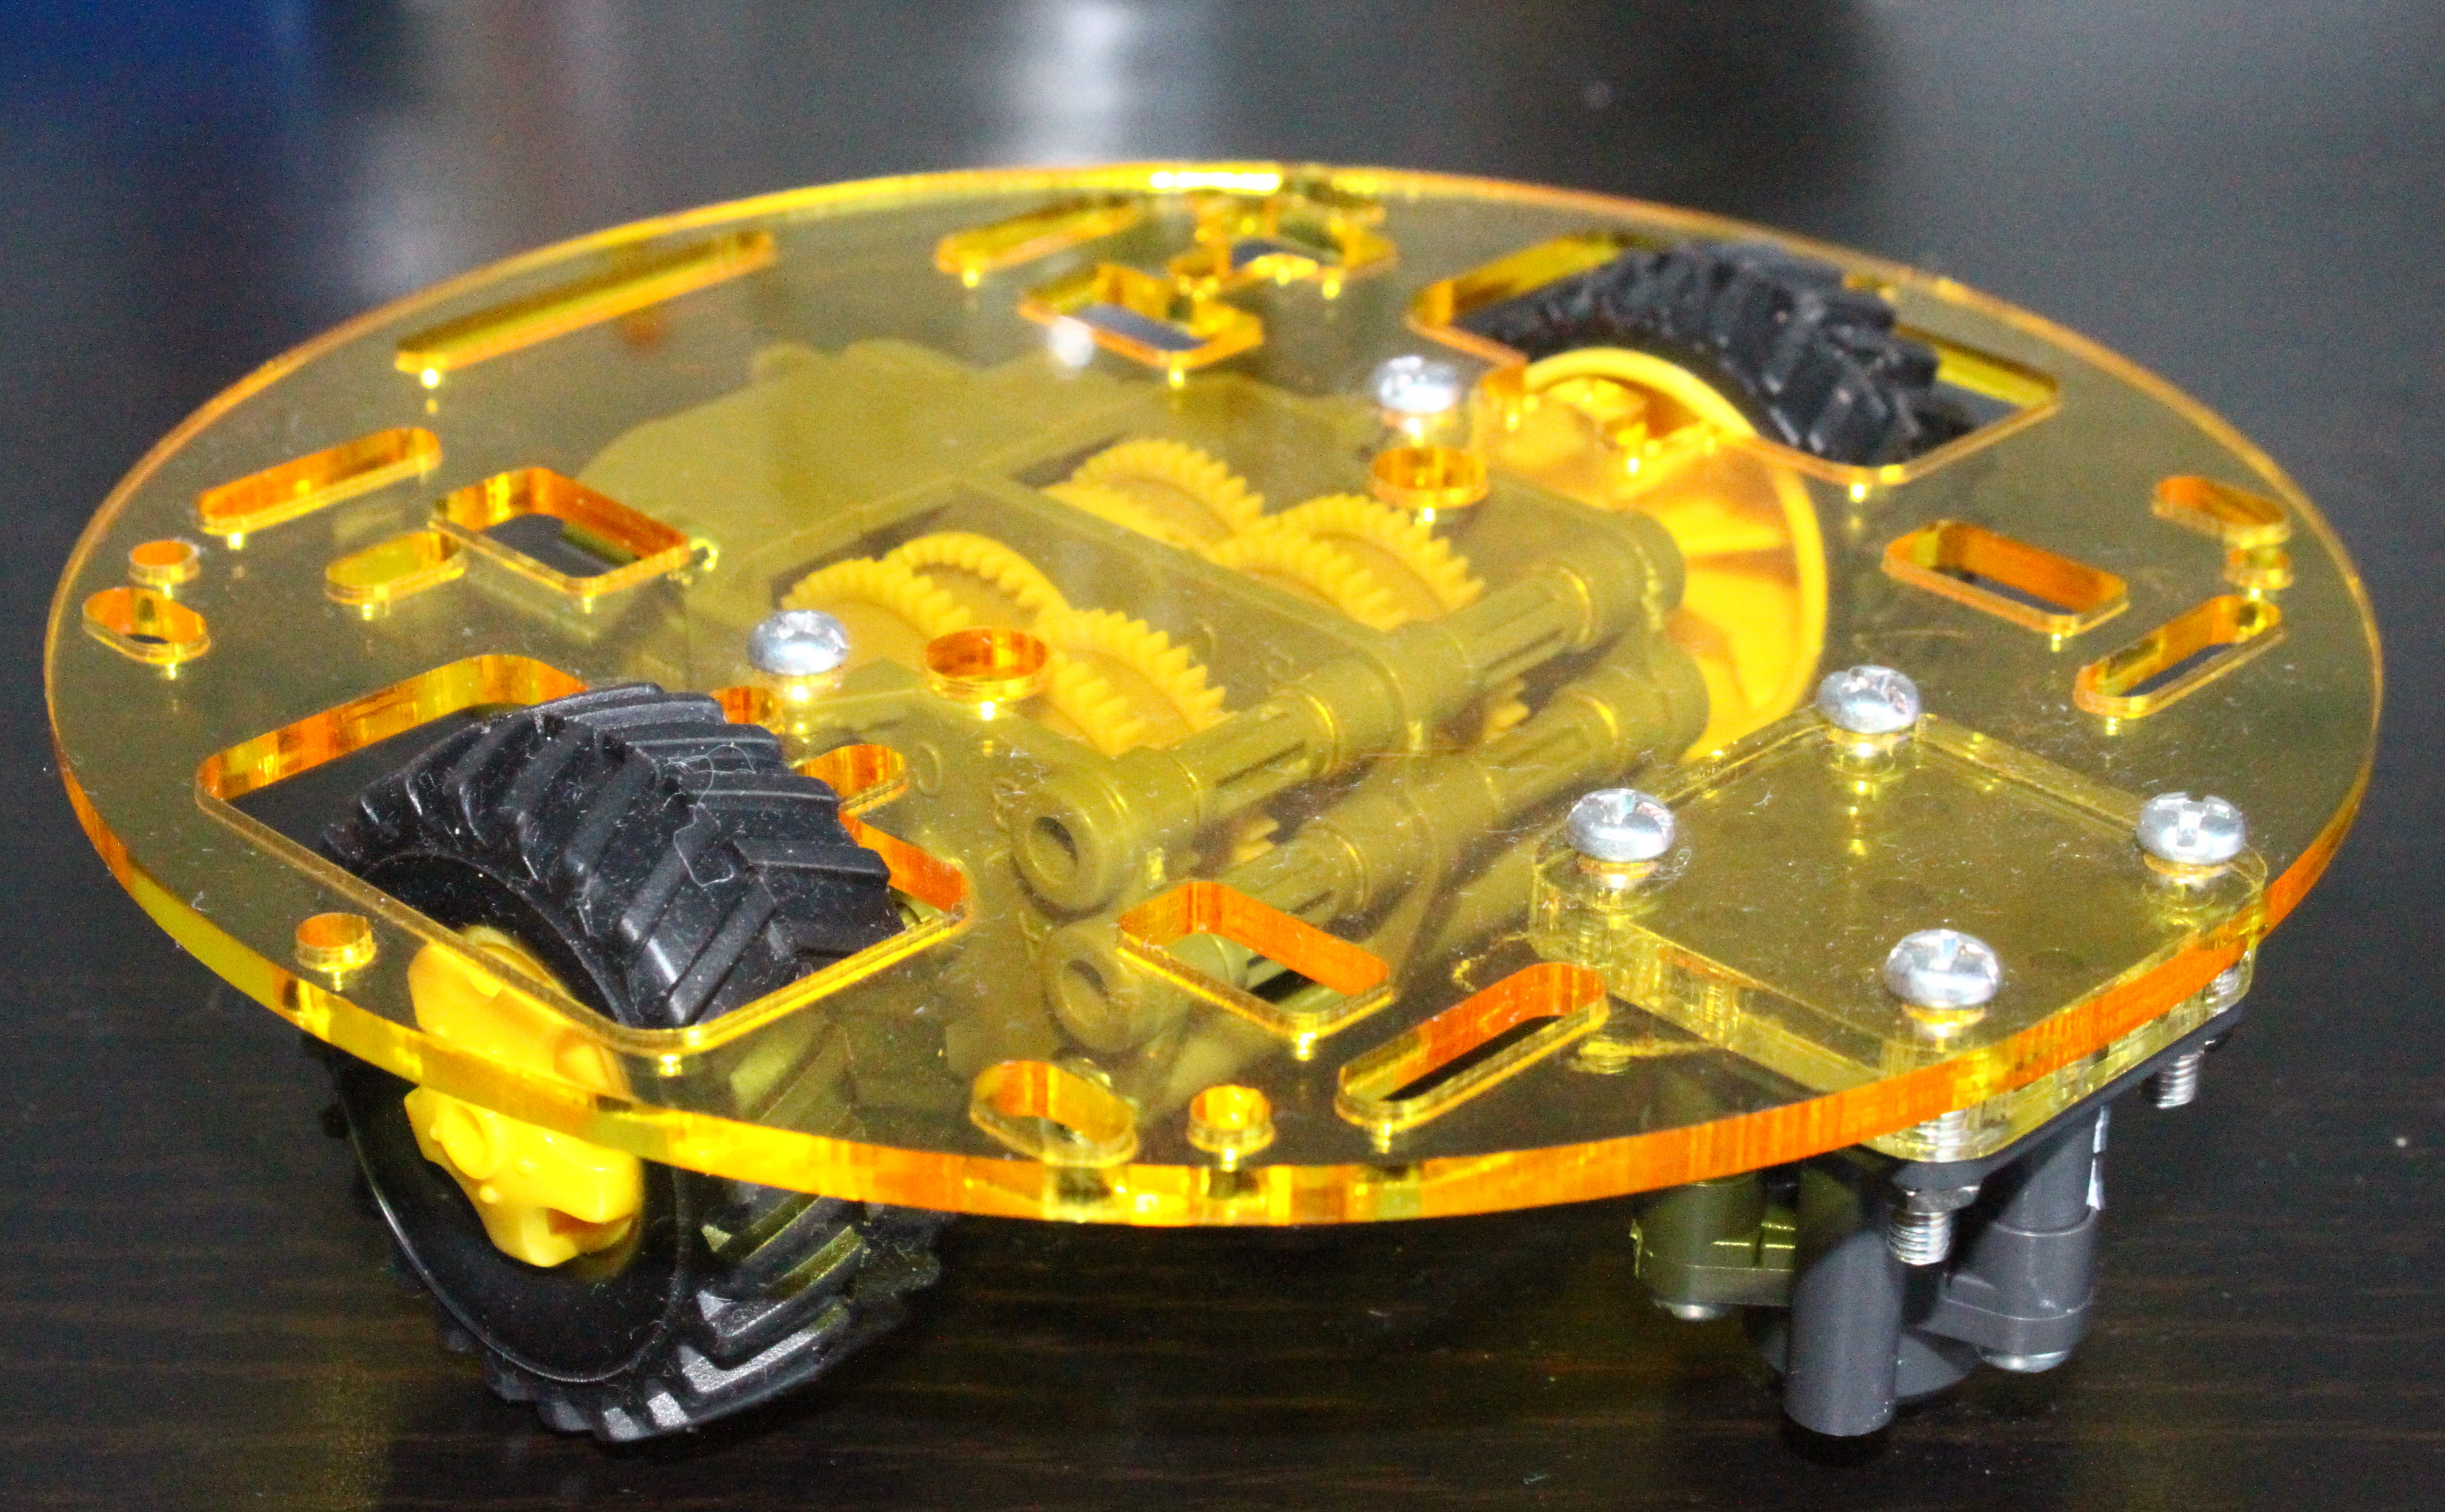
\includegraphics[width=\textwidth]{./Figures/RobotBase.jpg}
\caption{The base of the robot}
\label{fig:RobotBase}
\end{figure}

\section{Project Management}
In order to reduce the risk within the project, all aspects of potential issues are looked at and are summarised in table \ref{tab:risk}. A Gantt chart of how time will be spent can be seen in figure \ref{fig:Gantt}. 

The project will be designed in stages - first, gaining operation of all the basic sections; movement, image capturing, image detection algorithms etc. These will then be brought together once tested to create the final product. 
\begin{table}
\begin{tabular}{|p{6cm}|p{2cm}|p{6cm}|}\hline
Risk						&	Severity	&	Prevention \\ \hline
Parts not arriving on time	&	High		&	Order parts as early as possible \\
Project not fulfilling specification				&	High		&	Develop in stages to obtain functionality in parts. Ensure enough time is allocated to the project.	\\
PCB Design is incorrect		&	Medium		&	Check the design carefully and get second opinion \\
Failure of personal computer causing data loss & Low	& 	Keep back ups of all work on Devtrack Git repository and Dropbox.\\

\hline
\end{tabular}
\caption{A list of risks and the prevention steps taken to reduce their impact}
\label{tab:risk}
\end{table}

%% ----------------------------------------------------------------
%% Conclusions.tex
%% ---------------------------------------------------------------- 
\chapter{Conclusions and Further Work} \label{Chapter: Conclusions}
%\section{Conclusion}

%\inote{What I have accomplished}
This work has led to a tested device which is mobile and has the capability to perform stereoscopic image processing. The system has the following parts:

\begin{enumerate}
\item Motor driving
\item Stereoscopic Cameras
\item SD Card memory
\item SDRAM
\item Image Processing
\end{enumerate} 

The motor system is a simple, cheap method to move distances with reasonable accuracy. A better controller would allow variable speed and speed matching between motors. The system was shown to work to $4.5\%$ accuracy over a $300mm$ distance.

Stereo image pairs can be captured and stored on an SD card in a FAT32 file system. The SD card is also used for transferring images to and reading log files on a computer. Images are stored in QVGA format ($320px \times 240px$) as a Bitmap image. 

An additional 4MB of SDRAM memory is available to use on the robot allowing for large data arrays of the images to be kept in fast access RAM. The RAM is direct memory accessed (DMA) so operation is almost seamless from internal memory.

Multiple comparison algorithms have been investigated and compared using the same test images. It was clear that, although at a necessity of more computations, the normalised cross correlation is the best with regard to overall reliability. 

Range finding equations were then researched and derived, which use the characteristics of the camera and the separation distance between them to calculate distance to objects in view. The range finding capability was tested using MATLAB and it found that the system could not accurately calculate distances to objects. However, depth perception is possible even with low resolution cameras and small separation between them. A wide angle lens could be added to the system to more accurately measure distances but at the expense of reducing the maximum range.

The Fourier transform was also investigated and implemented. The system allows for a 2D array of a square image with dimensions of $2^{2n}\; $, where $n \in \mathbb{N}$, and is limited by RAM space and time. The transform is speed optimised and in tests proved to be fairly accurate. 

All aspects implemented on the robot have been shown to be functional. A faster processor would have been a good idea to use for image processing, but this could have developed other problems with the PCB. The Raspberry Pi or Steve Gunn's \textit{`L'Imperatrice'}, which both run a Linux operating system, would have been a good choice to remove the need for as much hardware design. Existing image processing libraries could then have been used to gain more functionality. 

Though some aspects of the specification were not fulfilled completely, the progress made during this project, and the challenges that have been overcome, provide a good platform for further development.
%Though the robots original application wasn't achieved, the end device is a base for a stereoscopic application. The system is a tested platform for future applications to be implemented on and additions can be made using the spare pins and bus connections on the PCB headers. 

The system could be used in future projects to develop more functionality. Wireless communications could be added to the system to allow a connection to the computer, and search algorithms can be implemented alongside distance calculations to make the robot aware of its surroundings. 
%\inote{What could be changed to make it better}
%\inote{Suggestions for further work}

\section{System Operation}

The system uses a debug USART available on J7 (57600bps, 8 data, 0 parity and 1 stop bit).

The system has two modes of operation, `Auto Run' and debug. By default, the Auto Run mode will run. Debug mode can be entered by the relevant command in the Auto Run procedure (see table \ref{table:AutoRun}) or by connecting Pin D23, available at Pin 1 of J9, to ground on system start. The state of the robot is shown by the LEDs. Table \ref{table:LEDs} shows the meaning of the LEDs.

Auto Run mode runs a set of commands located in \textit{``AutoRun.txt''} on the SD Card. If this file is not present, the system will run a default procedure defined in the code. A list of commands that can be run from this mode can be seen in table \ref{table:AutoRun}. The commands are specified by line. If an invalid command is found, the system will exit and run the \textit{System\_Error} loop. The  \textit{System\_Error} loop prints the status of all devices out once a second. By attaching a USART terminal, the error can be found.

Debug mode is a DOS-shell style terminal allowing the user to access methods and variables. This was used for development and debugging. A full list of commands can be seen in table \ref{table:Debug}. 

The final robot can be seen in figure \ref{fig:Robot:Complete}.

\begin{figure}
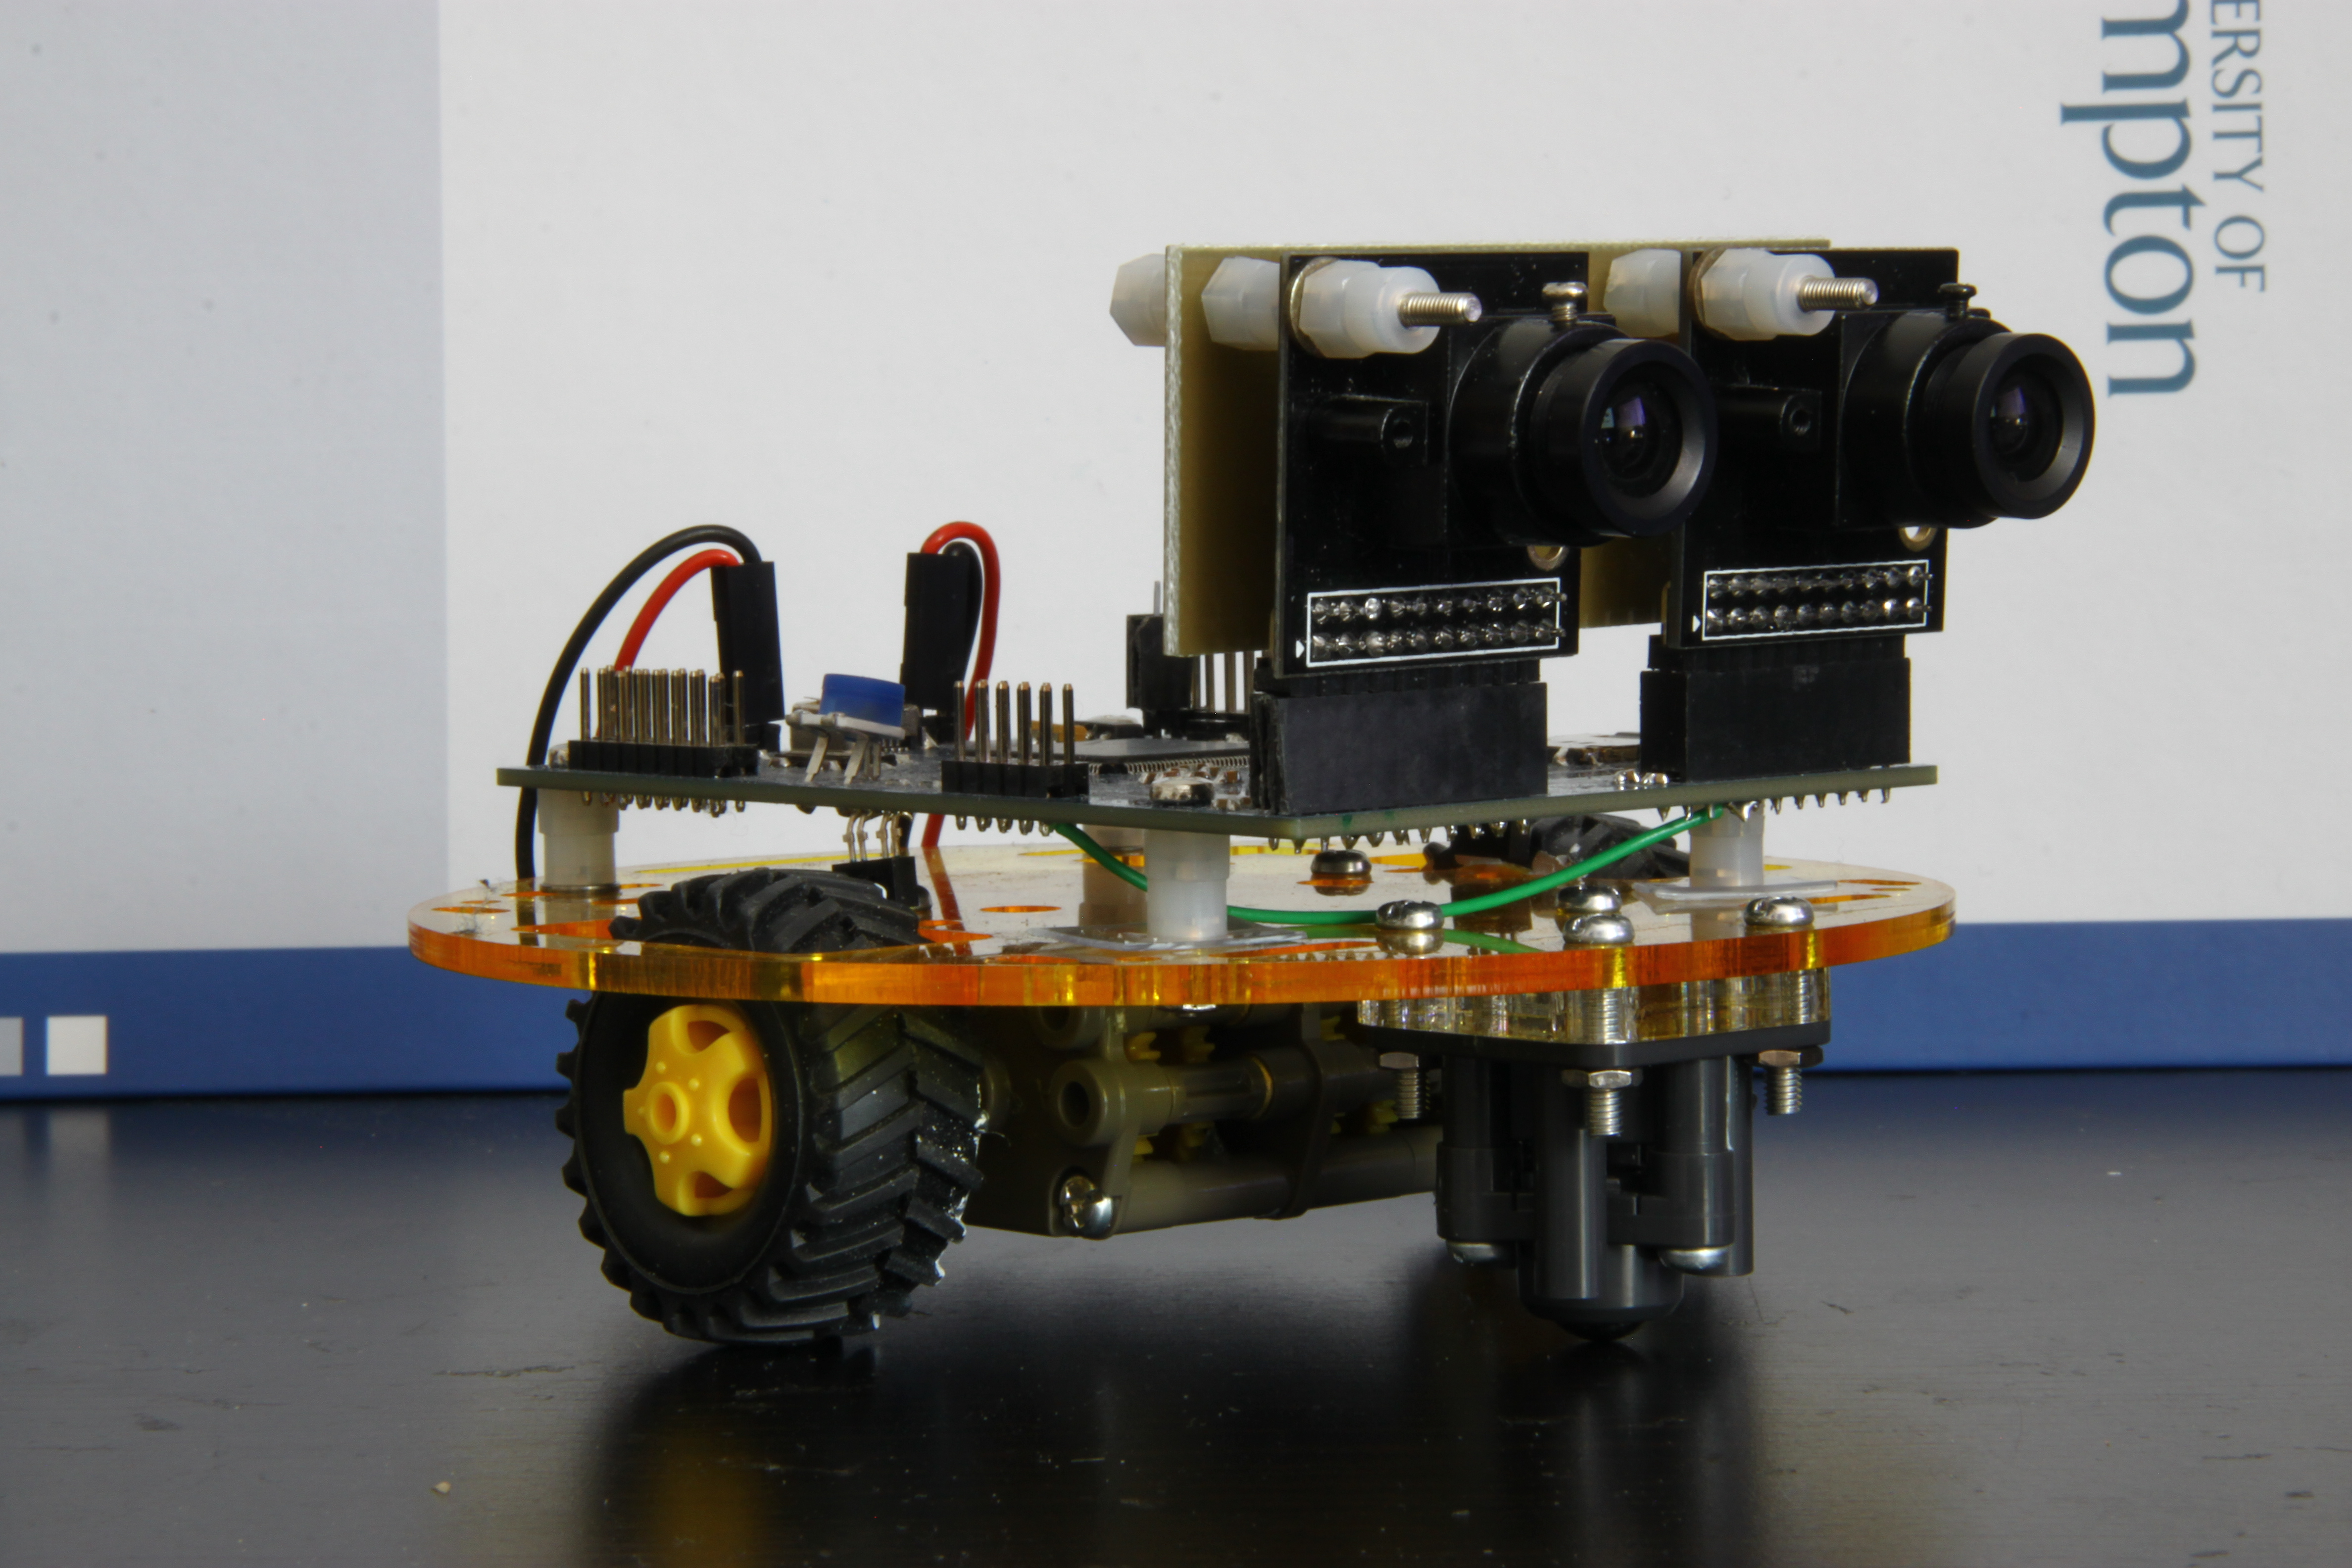
\includegraphics[width=\textwidth]{Figures/Robot.jpg}
\caption{The completed robot}
\label{fig:Robot:Complete}
\end{figure}

\begin{table}
\centering
\caption{Table showing the Auto Run commands implemented}
\label{table:AutoRun}
\begin{tabular}{ccc}\toprule
Command & 	Argument 			& 	Operation \\\toprule
B		&	int					&	Move backward by the argument value (millimetres) \\\midrule
F		&	int 				&	Move forward by the argument value (millimetres)\\\midrule
J		&	int					&	Jumps to the command specified (0 indexed)\\\midrule
P		&	N/A					&	Takes a stereo pair of photos\\\midrule
q		&	N/A					&	Quits Auto Run and enters debug mode\\\midrule
R		& 	int 			 	&	Rotates by argument (degrees)\\ \bottomrule
\end{tabular}
\end{table}

\begin{table}
\centering
\caption{Table showing the available debug commands}
\label{table:Debug}
\begin{tabular}{llp{10cm}}\toprule
Command & Argument & Operation \\\toprule
? && Shows the help prompt\\ \midrule
A && Runs the Auto Run procedure in debug mode\\ \midrule
B && Reads a Bitmap file and prints information \\ \midrule
c && converts the working buffer from integer to fixed point\\\midrule
C && Converts the working buffer from fixed point to integer\\\midrule
d && Saves the Working Buffer to ``Buffer\_results.csv'' \\ \midrule
D && Frees the Memory pointed to by the Working Buffer \\ \midrule
f && Reads ``Buffer.csv'' as a 2D Array of FFT\_SIZE by FFT\_SIZE\\ \midrule
g && Saves the Complex Buffer to ``Buffer\_Complex.csv'' \\\midrule
k && Prints the Complex Buffer \\ \midrule
m && Computes the Magnitude of the 1D FFT of the Working Buffer \\\midrule
M F &(int) & Drive Robot forward by (int) millimetres (negative number for reverse)\\\midrule
M L && Dive Left Wheel Forward a full rotation \\\midrule
M q && Resets Motors \\\midrule
M R && Drive Right Wheel Forward a full rotation \\\midrule
M T &(int) & Rotate Robot by (int) degrees (positive turns Clockwise)\\\midrule
o && Displays the fixed point value for (int)1 \\\midrule
P && Takes and stores Stereo Photos \\ \midrule
r && displays the contents of the working buffer\\\midrule
R && Reads contents of ``signal.bin'', representing 1D Signal. Integers, Big Endian\\\midrule
T && Reads contents of ``signal2d.bin'', representing 2D Signal. \\ \midrule
s && saves the working buffer\\\midrule
S && Saves the image in memory to a Bitmaps \\\midrule
v && Prints the status variables \\ \midrule
1 && computes the One Dimensional FFT of the working buffer. Returns magnitude.\\\midrule
2 && Computes the Magnitude of the Two Dimensional FFT of the Working Buffer. \\ \midrule
3 && Computes the Complex 2D FFT of the working buffer and stores it in the Complex Buffer \\ \bottomrule
\end{tabular}
\end{table}

\begin{table}
\centering
\caption{Table show the meaning of the LED lights. F - Flashing, X - Don't Care}
\label{table:LEDs}
\begin{tabular}{ccccccc}\toprule
\multicolumn{6}{c}{LED} 						& Meaning\\ \cmidrule{1-6}
MOTOR 	& 2		& 3 	& 4 	& 5 	& 6 	& \\ \toprule
Off		& Off	& Off	& Off	& Off	& Off	& System Initialising \\ \midrule
On		& X		& X		& X		& X		& X		& Robot moving\\\midrule
Off		& X		& X		& X		& X		& X		& Robot not moving\\\midrule
X		& On	& On	& On	& X		& X 	& System in Debug Mode \\\midrule
X		& X		& X		& X		& On	& X		& Left Wheel on a `Tab'	\\\midrule
X		& X		& X		& X		& Off	& X		& Left Wheel not on a `Tab'	\\\midrule
X		& X		& X		& X		& X 	& On	& Right Wheel on a `Tab'	\\\midrule
X		& X		& X		& X		& X		& Off	& Right Wheel not on a `Tab'	\\\midrule
Off		& On	& Off	& Off	& X		& X		& Auto Run Mode - Robot taking photos	\\\midrule
On		& Off	& On	& Off	& X		& X		& Auto Run Mode - Robot rotating	\\\midrule
On		& Off	& Off	& On	& X		& X		& Auto Run Mode - Robot moving\\\midrule
Off		& F		& Off	& Off	& X		& X		& System Error - Generic\\\midrule
Off		& F		& F		& X		& X		& X		& System Error - SD Card Error\\\midrule
Off		& F		& X		& F		& X		& X		& System Error - Camera Error\\ \bottomrule
\end{tabular}
\end{table}

\appendix
%% ----------------------------------------------------------------
%% AppendixA.tex
%% ---------------------------------------------------------------- 
\chapter{Circuit Diagrams} \label{Chapter:AppendixA:CircuitDiagrams}
\section{OV7670 Breakout Board Schematic}
\begin{figure}
\includegraphics[width=\textwidth,height=\textheight,keepaspectratio]{Figures/OV7670_Schematic.jpg} 
\caption{The circuit diagram for the OV7670 breakout board}
\label{OV7670_Schematic}

\end{figure}
\backmatter
\bibliographystyle{ecs}
%\bibliographystyle{unsrt}
\bibliography{ECS}
\end{document}
%% ----------------------------------------------------------------
